% !TeX encoding = UTF-8
% !TeX program = xelatex
% !TeX spellcheck = fr
% !TeX root = tm_astro_main.tex


\chapter{L'E-ELT}\label{4}

L'European Extremely Large Telescope est un télescope optique actuellement en cours de construction qui est développé par l'European Southern Observatory (ESO) depuis 2005. Comme son nom l'indique, il fait partie de la catégorie des Extremely Large Telescope (ELT). Cette classe contient tout les télescopes optiques possédant un miroir primaire de diamètre supérieur à 20 mètres. Il existe à ce jour 3 ELT en construction; leur mise en service respective est prévue entre 2024 et 2027. L'ELT qui nous intéresse dans ce travail, l'E-ELT, possède, avec ses 39.3 mètres, le plus grand miroir de la catégorie des télescopes géants et par extension le plus grand télescope optique jamais construit. Son lieu de construction à 3060 mètres d'altitude se situe à Cerro Armazones dans le désert d'Atacama au Chili. La taille de son miroir primaire ainsi que la faculté d'observer dans le spectre visible et l'infrarouge lui permettront d'éclairer de nombreuses zones d'ombre concernant des sujets tels que: les exoplanètes, la population stellaire des galaxies ou encore le cycle de vie des étoiles enrichissant le milieu interstellaire (§\ref{5}).

\begin{figure}[H]
	\centering
	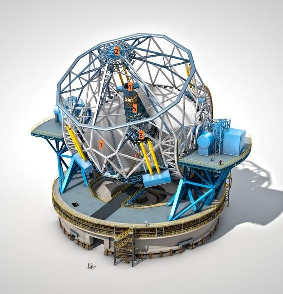
\includegraphics[scale=1.35]{images/e-elt_i}
	\caption[Vue d'artiste de l'E-ELT avec les 5 miroirs primaires \label{Fig. 4.1}\newline \url{https://fis-landschaft.de/universum/elt/}]{Vue d'artiste de l'E-ELT avec les 5 miroirs primaires \label{Fig. 4.1}}
	\label{Fig. 4.1}
\end{figure}

\section{Les raisons et les technologies nécessaires à la construction de l'E-ELT}\label{4.1}

Au fur et à mesure que la recherche scientifique en astronomie progresse, des télescopes de plus en plus performants sont nécessaires. Pour cela, il existe plusieurs manières d'accroître la qualité d'un télescope. L'une de ces manières consiste à augmenter la quantité de lumière collectée en grossissant le diamètre de l'instrument, cela permet d'augmenter la quantité de détails observés. Une autre des solutions réside dans l'augmentation de la qualité des différents instruments traitant l'image créée par le télescope. A ce jour, ces instruments ont atteint une qualité quasi-parfaite, donc la seule solution pour augmenter les performances des télescopes est d'en construire des plus gros. Cependant, il n'est pas si simple de fabriquer un miroir de 39 mètres et d'éviter des aspérités plus grandes que 150 $\mu m$ lors du polissage, de plus les contraintes qui agiraient sur le miroir seraient telles qu'il serait quasi-impossible de le construire. Pour contrer ce problème, le miroir de l'E-ELT ne sera pas construit en une seule pièce, il utilisera plutôt la technique du miroir segmenté. Cette technique, utilisée pour la première fois en 1979 avec le Multiple Mirror Telescope, consiste à remplacer un grand miroir par un grand nombre de plus petits miroirs assemblés les uns avec les autres. Ainsi, l'E-ELT sera composé de 798 miroirs hexagonaux de 1.44 mètres de côté, qui constitueront au total 5 grands miroirs primaires (Fig. \ref{Fig. 4.1}). L'E-ELT bénéficie encore d'une technologie récente permettant d'énormes progrès à l'observation terrestre, l'optique adaptative. Cette technologie a pour but de corriger les perturbations liées à l'atmosphère en utilisant 6 lasers qui l'analyseront en permanence. Ces-derniers seront couplés à un système de vérins qui pourront déformer les miroirs 4 et 5 pour compenser les turbulences atmosphériques jusqu'à 1000 fois par seconde.